\section{The physical equations behind GETM}

\subsection{Hydrodynamic equations}

\subsubsection{Three-dimensional momentum equations}\label{Section_3d_momentum}

For geophysical coastal sea 
and ocean dynamics, usually the three-dimensional hydrostatic equations
of motion with the Boussinesq approximation and the eddy 
viscosity assumption are used (\cite{BRYAN69}, \cite{COX84},
\cite{BLUMBERGea87}, \cite{HAIDVOGELea99}, \cite{KANTHAea00b}). 
In the flux form, the dynamic equations of motion for
the horizontal velocity components can be written in Cartesian
coordinates as:


\begin{equation}\label{uEq}
\begin{array}{l}
\displaystyle
\partial_t u
+\partial_z(uw)
-\partial_z\left((\nu_t+\nu) \partial_z u\right)
\\ \\ \displaystyle
\qquad+\alpha\bigg(\partial_x(u^2)+\partial_y(uv)
-\partial_x\left(2A_h^M\partial_xu\right)-\partial_y\left(A_h^M
(\partial_yu+\partial_xv)\right)
\\ \\ \displaystyle
\qquad
-fv
-\int_z^{\zeta}\partial_x b\,dz' \bigg)
=
- g\partial_x \zeta,
\end{array}
\end{equation}

\begin{equation}\label{vEq}
\begin{array}{l}
\displaystyle
\partial_t v +\partial_z(vw)
-\partial_z\left((\nu_t+\nu) \partial_z v\right)
\\ \\
\displaystyle
\qquad+\alpha\bigg(\partial_x(vu)+\partial_y(v^2)
-\partial_y\left(2A_h^M\partial_yv\right)-\partial_x\left(A_h^M
(\partial_yu+\partial_xv)\right)
\\ \\
\displaystyle
\qquad
+fu
-\int_z^{\zeta}\partial_x b\,dz' \bigg)=
- g\partial_y \zeta.
\end{array}
\end{equation}

The vertical velocity is calculated by means of the
incompressibility condition:

\begin{equation}\label{Konti}
\partial_x u +\partial_y v +\partial_z w = 0.
\end{equation}


Here, $u$, $v$ and $w$ are the ensemble averaged
velocity components with respect
to the $x$, $y$ and $z$ direction, respectively.
The vertical coordinate $z$ ranges from the bottom $-H(x,y)$ \label{Hxy}
to the surface $\zeta(t,x,y)$ with $t$ denoting time.
$\nu_t$ is the vertical eddy viscosity, $\nu$ the kinematic viscosity,
$f$ the Coriolis
parameter, and $g$ is the gravitational acceleration.
The horizontal mixing is parameterised by terms containing the
horizontal eddy viscosity $A_h^M$, see \cite{BLUMBERGea87}.  
The buoyancy $b$ is defined as

\begin{equation}\label{bdef}
b=-g\frac{\rho-\rho_0}{\rho_0}
\end{equation}

with the density $\rho$ and a reference density $\rho_0$.
The last term on the left hand sides of equations (\ref{uEq}) and (\ref{vEq})
are the internal (due to density gradients)
and the terms on the right hand sides are the external
(due to surface slopes) pressure gradients. In the latter, the deviation of
surface density from reference density is neglected (see \cite{BURCHARDea97}).
The derivation of equations (\ref{uEq}) - (\ref{Konti}) has been shown in
numerous publications, see e.g.\ \cite{PEDLOSKY87}, \cite{HAIDVOGELea99},
\cite{BURCHARD02}.

In hydrostatic 3D models, the vertical velocity is calculated by means of
equation (\ref{Konti}) velocity equation. 
Due to this, mass conservation and free surface elevation
can easily be obtained.

Drying and flooding of mud-flats is already incorporated in
the physical equations by multiplying some terms with the
non-dimensional number $\alpha$ which equals unity in regions where a
critical water depth $D_{crit}$ is exceeded and approaches zero
when the water depth $D$ tends to a minimum value $D_{min}$:

\begin{equation}\label{alpha}
\alpha=\min\left\{1,\frac{D-D_{min}}{D_{crit}-D_{min}}\right\}.
\end{equation}

Thus, $\alpha=1$ for $D\geq D_{crit}$,  such that the usual momentum
equation results except for very shallow water, where simplified physics
are considered with a balance between tendency, friction and external pressure
gradient. In a typical wadden sea application, $D_{crit}$ is of the order
of 0.1 m and $D_{\min}$ of the order of 0.02 m (see \cite{BURCHARD98},
\cite{BURCHARDea03a}). 


\subsubsection{Kinematic boundary conditions and surface elevation equation}

At the surface and at the bottom, kinematic boundary conditions
result from the requirement that 
the particles at the boundaries are moving along these boundaries:

\begin{equation}\label{KinBoundsSurf}
w= \partial_t \zeta +  u \partial_x\zeta + v \partial_y \zeta
\qquad \mbox{for } z=\zeta,
\end{equation}

\begin{equation}\label{KinBoundsBott}
w= - u \partial_xH - v \partial_y H
\qquad \mbox{for } z=-H.
\end{equation}

\subsubsection{Dynamic boundary conditions}\label{SectionDynBounds}

At the bottom boundaries, no-slip conditions are prescribed for the horizontal
velocity components:

\begin{equation}\label{DynBoundbx}
u=0, \quad v=0.
\end{equation}

With (\ref{KinBoundsBott}), also $w=0$ holds at the bottom.
It should be noted already here, that the bottom boundary condition
(\ref{DynBoundbx}) is generally not directly used in numerical ocean models,
since the near-bottom values of the horizontal velocity components
are not located at the bed, but half a grid box above it.
Instead, a logarithmic velocity profile is assumed in the bottom layer,
leading to a quadratic friction law, see section \ref{sec-bottom-friction-3d}.

At the surface, the dynamic boundary conditions read:

\begin{equation}\label{DynBoundSx}
\begin{array}{l}
(\nu_t+\nu) \partial_z u=\alpha \tau^x_{s},
\\ \\
(\nu_t+\nu) \partial_z v=\alpha \tau^y_{s},
\end{array}
\end{equation}

The surface stresses (normalised by the reference density) $\tau_s^x$
and $\tau_s^y$ are calculated as functions of wind speed, wind direction,
surface roughness etc.
Also here, the drying parameter $\alpha$ is included in order to
provide an easy handling of drying and flooding.

\subsubsection{Lateral boundary conditions}

Let $G$\label{G} denote the lateral boundary of the model domain with the
closed land boundary $G^c$\label{Gc} and the open boundary $G^o$\label{Go} such that
$G^c \cup G^o=G$ and $G^c \cap G^o=\emptyset$.  
Let further $\vec u=(u,v)$\label{vecu} denote the horizontal velocity vector
and $\vec u_n=(-v,u)$\label{vecun} its normal vector.  
At closed boundaries, the flow must be parallel to the boundary:

\begin{equation}
\vec u_n \cdot \vec\nabla G^c = 0 
\end{equation}

with $\vec\nabla=(\partial_x,\partial_y)$ being the gradient operator.

For an eastern or a western closed boundary with
$\vec\nabla G^c=(0,1)$ this has the consequence that
$u=0$ and, equivalently, for a southern
or a northern closed boundary with $\vec\nabla G^c=(1,0)$
this has the consequence that $v=0$.

At open boundaries, the velocity gradients across the boundary vanish:

\begin{equation}
\vec\nabla_n u \cdot \vec\nabla G^o = 0, \quad 
\vec\nabla_n v \cdot \vec\nabla G^o = 0, \quad 
\end{equation}

with $\vec\nabla_n=(-\partial_y,\partial_x)$ being the 
operator normal to the gradient operator.

For an eastern or a western open boundary with
this has the consequence that
$\partial_x u=\partial_x v =0$ and, equivalently, for a southern
or a northern open boundary
this has the consequence that $\partial_y u=\partial_y v =0$.

At so-called forced
open boundaries, the sea surface elevation $\zeta$ is prescribed. 
At passive open boundaries, it is assumed that the curvature of the
surface elevation normal to the boundary is zero, with the consequence that
the spatial derivatives of the surface slopes normal to the boundaries vanish. 

\subsection{GETM as slice model}\label{Section_GETM_Slice}

By chosing the compiler option {\tt SLICE\_MODEL} it is possible to
operate GETM as a two-dimensional vertical ($xz$-)model under the assumption
that all gradients in $y$-direction vanish. In order to do so,
a bathymetry file with a width of 4 grid points has to be generated,
with the outer ($j=1$, $j=4$) bathymetry values set to land, and the two inner
ones being independent on $j$. The compiler option {\tt SLICE\_MODEL}
then sets the transports, velocities, and sea surface elevations such that
they are independent of $y$, i.e.\ they are forced to be identical for
the same $j$-index. Especially, the $V$-transports and velocities 
in the walls ($j=1$, $j=3$) are set to the calculated value at index
$j=2$.

\section{Transformations}\label{SectionTransformations} 

\subsection{General vertical coordinates}\label{SectionGeneralCoordinates}  

As a preparation of the discretisation, the physical space
is vertically divided into $N$ layers. This is done by introducing
internal surfaces $z_k$, $k=1,\dots,N-1$
which do not intersect,
each depending on the horizontal position $(x,y)$ and time $t$.
Let

\begin{equation}\label{gamma_def}
-H(x,y)=z_0(x,y)<z_1(x,y,t)<\dots<z_{N-1}(x,y,t)<z_N(x,y,t)=\zeta(x,y,t)
\end{equation}
define the local layer depths $h_k$ with

\begin{equation}\label{hkdef}
h_k=z_k-z_{k-1}.
\end{equation}
for $1\leq k\leq N$. For simplicity, the argument $(x,y,t)$ is omitted in
most of the cases.

The most simple layer distribution is given by the so-called $\sigma$
\label{sigmacoord} transformation 
(see \cite{PHILLIPS57} for a first application
in meteorology and \cite{FREEMANea72} for a first application
in hydrodynamics) with

\begin{equation}\label{sigma}
\sigma_k=\frac{k}{N}-1 
\end{equation}

and 

\begin{equation}\label{sigmaz}
z_k=D\sigma_k 
\end{equation}
for $0\leq k\leq N$.

The $\sigma$-coordinates can also be refined towards the surface and the
bed:

\begin{equation}\label{formula_Antoine}
\beta_k = \frac{\mbox{tanh}\left( (d_l+d_u)(1+\sigma_k)-d_l\right)
+\mbox{tanh}(d_l)}{\mbox{tanh}(d_l)+\mbox{tanh}(d_u)}-1,
\qquad k=0,\dots,N\qquad
\end{equation}

such that $z$-levels are obtained as follows:

\begin{equation}
z_k=D\beta_k 
\end{equation}
for $0\leq k\leq N$.

The grid is refined towards the surface for $d_u>0$ and refined towards
the bottom for $d_l>0$. When both, $d_u$ and $d_l$ are larger than zero,
then refinement towards surface and bed is obtained. For 
$d_u=d_l=0$ the $\sigma$-transformation (\ref{sigma}) with
$\beta_k=\sigma_k$ is retained. 
Figure \ref{FigGeneral1} shows four examples for vertical layer
distributions obtained with the $\sigma$-transformation. 

Due to the fact that all layer thicknesses are proportional to
the water depth, 
the equidistant and also the non-equidistant $\sigma$-transformations,
(\ref{sigma}) and (\ref{formula_Antoine}), 
have however one striking disadvantage. In order to 
sufficiently resolve the mixed layer also in deep water, many
layers have to be located near the surface. 
The same holds for the bottom boundary layer. 
This problem of $\sigma$-coordinates has been discussed by
several authors (see e.g.\ \cite{DELEERSNIJDERea92}, \cite{KOK92},
\cite{GERDES93}, \cite{SONGea94},
\cite{BURCHARDea97}) who suggested methods
for generalised vertical coordinates not resulting in layer 
thicknesses not proportional to the water depth. 

The generalised vertical coordinate introduced here is a
generalisation of the so-called mixed-layer transformation
suggested by \cite{BURCHARDea97}. It is a hybrid coordinate which
interpolates between the equidistant and the
non-equidistant $\sigma$-transformations given by 
(\ref{sigma}) and (\ref{formula_Antoine}). The weight for the interpolation
depends on the ratio of a critical water depth $D_{\gamma}$ (below which
equidistant $\sigma$-coordinates are used) and the actual water depth:

\begin{equation}\label{HJVTrans}
z_k = D\left(\alpha_{\gamma} \sigma_k + (1-\alpha_{\gamma}) \beta_k\right) 
\end{equation}

with 

\begin{equation}\label{MLDTransform}
\alpha_{\gamma} = \min\left(\frac{
(\beta_k-\beta_{k-1})-\frac{D_{\gamma}}{D}(\sigma_k-\sigma_{k-1})}
{(\beta_k-\beta_{k-1})-(\sigma_k-\sigma_{k-1})},1\right).
\end{equation}

and $\sigma_k$ from (\ref{sigma}) and  $\beta_k$ from (\ref{formula_Antoine}). 

For inserting $k=N$ in (\ref{MLDTransform}) and $d_l=0$ and $d_u>0$
in (\ref{formula_Antoine}), 
the mixed layer transformation of 
\cite{BURCHARDea97} is retained, see the upper two
panels in figure \ref{FigGeneral2}. 
Depending on the values for 
$D_{\gamma}$ and  $d_u$, some near-surface layer thicknesses
will be constant in time and space, allowing for
a good vertical resolution in the surface mixed layer. 

The same is obtained for the bottom with the following settings:
$k=1$, $d_l>0$ and $d_u=0$, see the lower two
panels in figure \ref{FigGeneral2}. This is recommended for reproducing 
sedimentation dynamics and other benthic processes.
For $d_l=d_u>0$ and $k=1$ or $k=N$ a
number of layers near the surface and near the bottom can be
fixed to constant thickness. 
Intermediate states are obtained by intermediate settings,
see figure \ref{FigGeneral3}. 
Some pathological
settings are also possible, such as $k=1$, $d_l=1.5$ and $d_u=5$,
see figure \ref{FigGeneral4}. 


\begin{figure}
\begin{center}
\psfrag{X}[cc][][0.6]{$x$ / nm}
\psfrag{Y}[cc][][0.6]{$z$ / m}
\psfrag{T}[cc][][0.8]{$\sigma$-coordinates, $d_u=0$, $d_l=0$}
\includegraphics[width=7cm,bbllx=50,bblly=50,bburx=529,bbury=346]{./figures/sigma.ps}
\psfrag{T}[cc][][0.8]{$\sigma$-coordinates, $d_u=1.5$, $d_l=0$}
\includegraphics[width=7cm,bbllx=50,bblly=50,bburx=529,bbury=346]{./figures/beta10.ps}
\psfrag{T}[cc][][0.8]{$\sigma$-coordinates, $d_u=0$, $d_l=1.5$}
\includegraphics[width=7cm,bbllx=50,bblly=50,bburx=529,bbury=346]{./figures/beta01.ps}
\psfrag{T}[cc][][0.8]{$\sigma$-coordinates, $d_u=1.5$, $d_l=1.5$}
\includegraphics[width=7cm,bbllx=50,bblly=50,bburx=529,bbury=346]{./figures/beta11.ps}
\caption{
$\sigma$-transformation with four different zooming options. The plots
show the 
vertical layer distribution for a cross section through the North Sea
from Scarborough in England to Esbjerg in Denmark. The shallow area at
about $x=100$ nm is the Doggerbank. 
}\label{FigGeneral1}
\end{center}
\end{figure}

\begin{figure}
\begin{center}
\psfrag{X}[cc][][0.6]{$x$ / nm}
\psfrag{Y}[cc][][0.6]{$z$ / m}
\psfrag{T}[cc][][0.8]{upper $\gamma$-coordinates, $d_u=1.5$, $d_l=0$}
\includegraphics[width=7cm,bbllx=50,bblly=50,bburx=529,bbury=346]{./figures/gammaup1.ps}
\psfrag{T}[cc][][0.8]{upper $\gamma$-coordinates, $d_u=5$, $d_l=0$}
\includegraphics[width=7cm,bbllx=50,bblly=50,bburx=529,bbury=346]{./figures/gammaup5.ps}
\psfrag{T}[cc][][0.8]{lower $\gamma$-coordinates, $d_u=0$, $d_l=1.5$}
\includegraphics[width=7cm,bbllx=50,bblly=50,bburx=529,bbury=346]{./figures/gammalow1.ps}
\psfrag{T}[cc][][0.8]{lower $\gamma$-coordinates, $d_u=0$, $d_l=5$}
\includegraphics[width=7cm,bbllx=50,bblly=50,bburx=529,bbury=346]{./figures/gammalow5.ps}
\caption{
Boundary layer transformation (or $\gamma$ transformation)
with concentration of layers in the surface mixed layer (upper two
panels) and with concentration of layers in the bottom mixed layer (lower two
panels). The critical depth $D_{\gamma}$ is here set to 20 m,
such that at all shallower depths the equidistant $\sigma$-transformation
is used. The same underlying bathymetry as in figure \ref{FigGeneral1} 
has been used. 
}\label{FigGeneral2}
\end{center}
\end{figure}

\begin{figure}
\begin{center}
\psfrag{X}[cc][][0.6]{$x$ / nm}
\psfrag{Y}[cc][][0.6]{$z$ / m}
\psfrag{T}[cc][][0.8]{upper $\gamma$-coordinates, $d_u=5$, $d_l=1.5$}
\includegraphics[width=7cm,bbllx=50,bblly=50,bburx=529,bbury=346]{./figures/gammauplow.ps}
\psfrag{T}[cc][][0.8]{lower $\gamma$-coordinates, $d_u=1.5$, $d_l=5$}
\includegraphics[width=7cm,bbllx=50,bblly=50,bburx=529,bbury=346]{./figures/gammalowup.ps}
\psfrag{T}[cc][][0.8]{symmetric $\gamma$-coordinates, $d_u=1.5$, $d_l=1.5$}
\includegraphics[width=7cm,bbllx=50,bblly=50,bburx=529,bbury=346]{./figures/gammauplow1.ps}
\psfrag{T}[cc][][0.8]{symmetric $\gamma$-coordinates, $d_u=5$, $d_l=5$}
\includegraphics[width=7cm,bbllx=50,bblly=50,bburx=529,bbury=346]{./figures/gammauplow5.ps}
\caption{
Boundary layer transformation (or $\gamma$ transformation)
with concentration of layers in both, 
the surface mixed layer and
the bottom mixed layer.  Four different realisations are shown. 
The critical depth $D_{\gamma}$ is here set to 20 m,
such that at all shallower depths the equidistant $\sigma$-transformation
is used.
The same underlying bathymetry as in figure \ref{FigGeneral1} 
has been used. 
}\label{FigGeneral3}
\end{center}
\end{figure}

\begin{figure}
\begin{center}
\psfrag{X}[cc][][0.6]{$x$ / nm}
\psfrag{Y}[cc][][0.6]{$z$ / m}
\psfrag{T}[cc][][0.8]{upper $\gamma$-coordinates, $d_u=1.5$, $d_l=5$}
\includegraphics[width=7cm,bbllx=50,bblly=50,bburx=529,bbury=346]{./figures/gammapathoup.ps}
\psfrag{T}[cc][][0.8]{lower $\gamma$-coordinates, $d_u=5$, $d_l=1.5$}
\includegraphics[width=7cm,bbllx=50,bblly=50,bburx=529,bbury=346]{./figures/gammapatholow.ps}
\caption{
Two pathological examples for the 
boundary layer transformation.
The critical depth $D_{\gamma}$ is here set to 20 m,
such that at all shallower depths the equidistant $\sigma$-transformation
is used.
The same underlying bathymetry as in figure \ref{FigGeneral1} 
has been used. 
}\label{FigGeneral4}
\end{center}
\end{figure}

The strong potential of the general vertical coordinates concept is the 
extendibility towards vertically adaptive grids. Since the layers
may be redistributed after every baroclinic time step, one could adapt the
coordinate distribution to the internal dynamics of the flow. One could
for example concentrate more layers at vertical locations of high
stratification and shear, or force certain layer interfaces towards
certain isopycnals, or approximate Lagrangian vertical coordinates by
minimising the vertical advection through layer interfaces. The advantages
of this concept have recently been demonstrated for one-dimensional water
columns by \cite{BURCHARDea04}. The three-dimensional generalisation
of this concept of adaptive grids for GETM is currently under
development.

\subsection{Layer-integrated equations}\label{SectionLayerIntegrated} 

There are two different ways to derive the layer-integrated
equations. \cite{BURCHARDea97} transform first the
equations into general vertical coordinate form
(see \cite{DELEERSNIJDERea92})
and afterwards
integrate the transformed equations over constant intervals in
the transformed space. \cite{LANDERea94} integrate the
equations in the Cartesian space over surfaces $z_k$ by
considering the Leibniz rule

\begin{equation}\label{Leibniz}
\int_{z_{k-1}}^{z_k}\partial_x f\,dz
=
\partial_x\int_{z_{k-1}}^{z_k} f\,dz
-f(z_k)\partial_xz_k
+f(z_{k-1})\partial_xz_{k-1}
\end{equation}

for any function $f$.
For the vertical staggering of the layer notation see figure
\ref{figvertgrid}.

More details about the layer integration are given in
\cite{BURCHARDea97}.

With the further definitions of layer integrated transport,

\begin{equation}\label{pqdef} 
p_k:=\int_{z_{k-1}}^{z_k}u\,dz,\qquad
q_k:=\int_{z_{k-1}}^{z_k}v\,dz,
\end{equation}

layer mean velocities,

\begin{equation}\label{ukvkdef} 
u_k:=\frac{p_k}{h_k},\qquad v_k:=\frac{q_k}{h_k},
\end{equation}

and layer averaged tracer concentrations and buoyancy,

\begin{equation}\label{ckbkdef} 
c^i_k:=\frac{1}{h_k}\int_{z_{k-1}}^{z_k}c^i\,dz,\qquad
b_k:=\frac{1}{h_k}\int_{z_{k-1}}^{z_k}b\,dz,
\end{equation}

and the grid related vertical velocity,

\begin{equation}\label{barwdef} 
\bar w_k:=(w-\partial_tz-u\partial_xz-v\partial_yz)_{z=z_k},
\end{equation}

the continuity equation (\ref{Konti}) has the layer-integrated form:

\begin{equation}\label{ContiLayerInt}
\partial_t h_k + \partial_x p_k + \partial_y q_k + \bar w_k - \bar w_{k-1}=0.
\end{equation}

It should be noted that the grid related velocity is located on the 
layer interfaces. 
After this, the layer-integrated momentum equations read as:

\begin{equation}\label{uEqvi}
\begin{array}{l}
\partial_t p_k 
+\bar w_k \tilde u_k -\bar w_{k-1} \tilde u_{k-1} 
-\tau^x_k + \tau^x_{k-1} 
\\ \\ \quad
+\alpha\Bigg\{\partial_x(u_kp_k)+\partial_y(v_kp_k)
\\ \\ \displaystyle \quad 
-\partial_x\left(2A_k^Mh_k\partial_xu_k\right)-\partial_y\left(A_k^Mh_k
(\partial_yu_k+\partial_xv_k)\right)
- fq_k 
\\ \\ \quad
\displaystyle
-h_k\left(
\frac12h_N(\partial^*_xb)_N
+\sum_{j=k}^{N-1}\frac12(h_j+h_{j+1})(\partial^*_xb)_j
\right)\Bigg\}
=
-gh_k\partial_x\zeta,
\end{array}
\end{equation}

\begin{equation}\label{vEqvi}
\begin{array}{l}
\partial_t q_k 
+\bar w_k  \tilde v_k -\bar w_{k-1}  \tilde v_{k-1} 
-\tau^y_k + \tau^y_{k-1} 
\\ \\ \quad
+\alpha\Bigg\{\partial_x(u_kq_k)+\partial_y(v_kq_k)
\\ \\ \displaystyle \quad 
-\partial_y\left(2A_k^Mh_k\partial_yv_k\right)-\partial_x\left(A_k^Mh_k
(\partial_yu_k+\partial_xv_k)\right)
+ fp_k 
\\ \\ \quad
\displaystyle
-h_k\left(
\frac12h_N(\partial^*_yb)_N
+\sum_{j=k}^{N-1}\frac12(h_j+h_{j+1})(\partial^*_yb)_j
\right)\Bigg\}
=
-gh_k\partial_y\zeta
\end{array}
\end{equation}

with suitably chosen advective horizontal 
velocities $\tilde u_k$ and $\tilde v_k$
(see section \ref{sec-uv-advect-3d}) on page \pageref{sec-uv-advect-3d}, 
the shear stresses

\begin{equation}\label{tauxkdef}
\tau^x_k = \left(\nu_t \partial_z u \right)_k,
\end{equation}

and 

\begin{equation}\label{tauykdef}
\tau^y_k = \left(\nu_t \partial_z v \right)_k,
\end{equation}

and the horizontal buoyancy gradients

\begin{equation}
(\partial^*_xb)_k=\frac12(\partial_xb_{k+1}+\partial_x b_k)
-\partial_xz_k\frac{b_{k+1}-b_k}{\frac12(h_{k+1}+h_k)}
\end{equation}

and 

\begin{equation}
(\partial^*_yb)_k=\frac12(\partial_yb_{k+1}+\partial_y b_k)
-\partial_yz_k\frac{b_{k+1}-b_k}{\frac12(h_{k+1}+h_k)}.
\end{equation}

The layer integration of the pressure gradient force 
is discussed in detail by \cite{BURCHARDea97}.

A conservative formulation can be derived 
for the recalculation of the physical vertical velocity
$w$ which is convenient
in the discrete space if $w$ is evaluated at the layer centres
(see \cite{DELEERSNIJDERea92}):

\begin{equation}\label{conservative_w}
w_k=\frac{1}{h_k}\left(
\partial_t(h_kz_{k-1/2})+\partial_x(p_kz_{k-1/2})+\partial_y(q_kz_{k-1/2})
+\bar w_kz_k-\bar w_{k-1}z_{k-1}\right).
\end{equation}

It should be mentioned that $w$ only needs to be evaluated for
post-processing reasons.

For the layer-integrated tracer concentrations, we obtain 
the following expression:

\begin{equation}\label{C_Layer_Int}
\begin{array}{l}
\partial_t (h_k c^i_k) + \partial_x (p_kc^i_k)+\partial_y (q_k c^i_k)
+(\bar w_k+w^s_k) \tilde c^i_k 
- (\bar w_{k-1}+w^s_{k-1}) \tilde c^i_{k-1}\\
\\ \qquad
-(\nu'_t\partial_z c^i)_{k}
+(\nu'_t\partial_z c^i)_{k-1}
-\partial_x\left(A_k^Th_k\partial_xc^i_k\right)
-\partial_y\left(A_k^Th_k\partial_yc^i_k\right)
=Q^i_k.
\end{array}
\end{equation}

It should be noted that the "horizontal" diffusion does no longer occur 
along geopotential surfaces but along horizontal coordinate lines.
The properly transformed formulation would include some cross-diagonal
terms which may lead to numerical instabilities due to violation
of monotonicity. For an in-depth discussion of this
problem, see \cite{BECKERSea98} and \cite{BECKERSea00}.   


\subsection{Horizontal curvilinear coordinates}\label{SectionCurviCoords} 

In this section, the layer-integrated equations from
section \ref{SectionTransformations} 
are transformed to horizontal orthogonal curvilinear 
coordinates. Similarly to general coordinates in the vertical,
these allow for much more flexibility when optimising 
horizontal grids to coast-lines and bathymetry. 
Furthermore, this type of coordinates system includes 
spherical coordinates as a special case. 
The derivation of the transformed equations is carried out here
according to \cite{HAIDVOGELea99}, see also \cite{ARAKAWAea77}. 

A rectangular domain with non-dimensional side lengths  
and with local Cartesian coordinates ${\cal X}$ and ${\cal Y}$
is mapped to a physical domain with four corners in such a way
that the local coordinates of the physical space,
$(\xi_x,\xi_y)$ are orthogonal to each others everywhere:

\begin{equation}\label{calXYdef} 
{\cal X} \rightarrow \xi_x,\quad {\cal Y} \rightarrow \xi_y. 
\end{equation}

The infinitesimal increments in the physical space,
$d\,\xi_x$ and $d\,\xi_y$ are related to the 
infinitesimal increments in the transformed space,
$d\,{\cal X}$ and $d\,{\cal Y}$ by so-called metric 
coefficients $m(x,y)$ and $n(x,y)$:

\begin{equation}\label{curvidef} 
d\,\xi_x = \left(\frac{1}{m} \right) d\,{\cal X}, \quad
d\,\xi_y = \left(\frac{1}{n} \right) d\,{\cal Y}. 
\end{equation}

These metric coefficients have the physical unit of [m$^{-1}$].  
With $m=n=$const, Cartesian coordinates are retained, and with

\begin{equation}\label{rE} 
m=\frac{1}{r_E\cos\phi},\quad n=\frac{1}{r_E},
\end{equation}

spherical coordinates with ${\cal X}=\lambda$\label{lambda}
and ${\cal Y}=\phi$
are retained 
(with the Earth's radius $r_E$, longitude $\lambda$ and
latitude $\phi$). 

With these notations, the layer-integrated equations 
(\ref{ContiLayerInt}), (\ref{uEqvi}), and (\ref{vEqvi}) given
in section \ref{SectionTransformations} can be formulated as 
follows: \\ 

{\bf Continuity equation:} 

\begin{equation}\label{ContiLayerIntCurvi}
\partial_t \left(\frac{h_k}{mn}\right) 
+ \partial_{\cal X} \left(\frac{p_k}{n} \right)
+ \partial_{\cal Y} \left(\frac{q_k}{m} \right)
+ \frac{\bar w_k - \bar w_{k-1}}{mn}=0.
\end{equation}

{\bf Momentum in $\xi_x$ direction:} 
\begin{equation}\label{uEqviCurvi}
\begin{array}{l}
\displaystyle 
\partial_t \left(\frac{p_k}{mn}\right)  
+\frac{\bar w_k \tilde u_k -\bar w_{k-1} \tilde u_{k-1}}{mn}  
-\frac{\tau^{\cal X}_k - \tau^{\cal X}_{k-1}}{mn}  
\\ \\ \quad
\displaystyle 
+\alpha\Bigg\{\partial_{\cal X}\left(\frac{u_kp_k}{n}\right)
+\partial_{\cal Y}\left(\frac{v_kp_k}{m}\right)
- q_k \left(\frac{f}{mn}+v_k\partial_{\cal X}\left(\frac{1}{n}\right)
-u_k\partial_{\cal Y}\left(\frac{1}{m}\right) \right)  
\\ \\ \quad
\displaystyle
-\partial_{\cal X}\left(\frac{2A_k^Mh_k}{n} m\partial_{\cal X}u_k\right)
-\partial_{\cal Y}\left(\frac{A_k^Mh_k}{m}
(n\partial_{\cal Y}u_k+m\partial_{\cal X}v_k)\right)
\\ \\ \quad
\displaystyle
-\frac{h_k}{n}\left(
\frac12h_N(\partial^*_{\cal X}b)_N
+\sum_{j=k}^{N-1}\frac12(h_j+h_{j+1})(\partial^*_{\cal X}b)_j
\right)\Bigg\}
=
-g\frac{h_k}{n}\partial_{\cal X}\zeta.
\end{array}
\end{equation}

{\bf Momentum in $\xi_y$ direction:} 
\begin{equation}\label{vEqviCurvi}
\begin{array}{l}
\displaystyle 
\partial_t \left(\frac{q_k}{mn}\right)  
+\frac{\bar w_k \tilde v_k -\bar w_{k-1} \tilde v_{k-1}}{mn}  
-\frac{\tau^{\cal Y}_k - \tau^{\cal Y}_{k-1}}{mn}  
\\ \\ \quad
\displaystyle 
+\alpha\Bigg\{\partial_{\cal X}\left(\frac{u_kq_k}{n}\right)
+\partial_{\cal Y}\left(\frac{v_kq_k}{m}\right)
+ p_k \left(\frac{f}{mn}+v_k\partial_{\cal X}\left(\frac{1}{n}\right)
-u_k\partial_{\cal Y}\left(\frac{1}{m}\right) \right)  
\\ \\ \quad
\displaystyle
-\partial_{\cal Y}\left(\frac{2A_k^Mh_k}{m} n\partial_{\cal Y}v_k\right)
-\partial_{\cal X}\left(\frac{A_k^Mh_k}{n}
(n\partial_{\cal Y}u_k+m\partial_{\cal X}v_k)\right)
\\ \\ \quad
\displaystyle
-\frac{h_k}{m}\left(
\frac12h_N(\partial^*_{\cal Y}b)_N
+\sum_{j=k}^{N-1}\frac12(h_j+h_{j+1})(\partial^*_{\cal Y}b)_j
\right)\Bigg\}
=
-g\frac{h_k}{m}\partial_{\cal Y}\zeta.
\end{array}
\end{equation}

In (\ref{uEqviCurvi}) and (\ref{vEqviCurvi}),
the velocity and momentum components $u_k$ and $p_k$
are now pointing into the $\xi_x$-direction and $v_k$ and $q_k$
are pointing into the $\xi_y$-direction. 
The stresses $\tau^{\cal X}_k$ and $\tau^{\cal Y}_k$
are related to these directions as well. 
In order to account for this rotation of the velocity and momentum vectors,
the rotational terms due to the Coriolis rotation are extended by 
terms related to the gradients of the metric coefficients. 
This rotation is here not considered for the horizontal diffusion terms in 
order not to unnecessarily complicate the equations. Instead we 
use the simplified formulation by \cite{KANTHAea00b}, who argue
that it does not make sense to use complex formulations for minor
processes with highly empirical parameterisations.  

Finally, the tracer equation is of the following form after
the transformation to curvilinear coordinates: 
\begin{equation}\label{C_Layer_IntCurvi}
\begin{array}{l}
\displaystyle
\partial_t \left(\frac{h_k c^i_k}{mn}\right) 
+ \partial_{\cal X} \left(\frac{p_kc^i_k}{n}\right)
+\partial_{\cal Y} \left(\frac{q_k c^i_k}{m}\right)
+\frac{\bar w_k \tilde c^i_k - \bar w_{k-1} \tilde c^i_{k-1}}{mn}\\
\\ \qquad
\displaystyle
-\frac{(\nu'_t\partial_z c^i)_{k}
-(\nu'_t\partial_z c^i)_{k-1}}{mn}
\\ \\ \qquad
\displaystyle
-\partial_{\cal X}\left(\frac{A_k^Th_k}{n} m\partial_{\cal X}c^i_k\right)
-\partial_{\cal Y}\left(\frac{A_k^Th_k}{m} n\partial_{\cal Y}c^i_k\right)
=\frac{Q^i_k}{mn}.
\end{array}
\end{equation}

\section{Discretisation}\label{Section_discretisation}

\subsection{Mode splitting}\label{Section_mode_splitting}

The external system consisting of the surface elevation equation
(\ref{Elevation}) and the transport equations (\ref{UMOM}) and
(\ref{VMOM}) underlies a strict time step constraint if the
discretisation is carried out explicitly:

\begin{equation}\label{CourantSurf}
\Delta t < \left[\frac12 \left(\frac{1}{\Delta x}+\frac{1}{\Delta y}\right)
\sqrt{2gD}\right]^{-1}.
\end{equation}

In contrast to that, the time step of the internal system
is only depending on the Courant number for advection,

\begin{equation}\label{CourantVel}
\Delta t < \min\left\{\frac{\Delta x}{u_{\max}},\frac{\Delta y}{v_{\max}}
\right\},
\end{equation}

which in the case of sub-critical flow is a much weaker
constraint. In order not to punish the whole model with a small
time step resulting from the external system, two different approaches
of mode splitting have been developed in the past.

The first approach, in which the external mode is calculated
implicitly, has been proposed by \cite{MADALAea77}.
This method
is numerically stable (if advection is absent)
for unconditionally long time steps.
The temporal approximation is of second order if semi-implicit
treatment is chosen. In such models, the external and internal mode are
generally calculated with the same time steps
(see e.g.\ \cite{BACKHAUS85}). The introduction of
interactions terms like (\ref{Slowfirst})
- (\ref{Slowlast}) is thus not necessary in such models.

Another approach is to use different time steps for the internal
(macro times steps $\Delta t$)
and the external mode \label{dtm} (micro time steps $\Delta t_m$).
One of the first free surface models which has adopted this method is the
Princeton Ocean Model (POM), see \cite{BLUMBERGea87}.
This method has the disadvantage that interaction
terms are needed for the external mode and that the consistency
between internal and external mode is difficult to obtain.
The advantage of this method is that the free surface elevation is
temporally well resolved which is a major requirement for models
including flooding and drying. That is the reason why this
method is adopted here.

The micro time step $\Delta t_m$ has to be an integer fraction $M$ of the
macro time step $\Delta t$. $\Delta t_m$ is limited by the speed of the
surface waves (\ref{CourantSurf}),
$\Delta t$ is limited by the current speed (\ref{CourantVel}).
The time stepping principle is shown in figure \ref{figtimegrid}.
The vertically integrated transports are averaged over each macro time
step:

\begin{equation}\label{Mdef} 
\bar U_{i,j}^{n+1/2} = \frac{1}{M}\sum_{l=n+0.5/M}^{n+(M-0.5)/M} U^l_{i,j}
\end{equation}
and
\begin{equation}
\bar V_{i,j}^{n+1/2} = \frac{1}{M}\sum_{l=n+0.5/M}^{n+(M-0.5)/M} V^l_{i,j}
\end{equation}
such that
\begin{equation}
\begin{array}{l}
\displaystyle
\frac{\zeta_{i,j}^{n+1}-\zeta_{i,j}^{n}}{\Delta t}=
-\frac{\bar U_{i,j}^{n+1/2}-\bar U_{i-1,j}^{n+1/2}}{\Delta x}
-\frac{\bar V_{i,j}^{n+1/2}-\bar V_{i,j-1}^{n+1/2}}{\Delta y}.
\end{array}
\end{equation}


\begin{figure}
\begin{center}
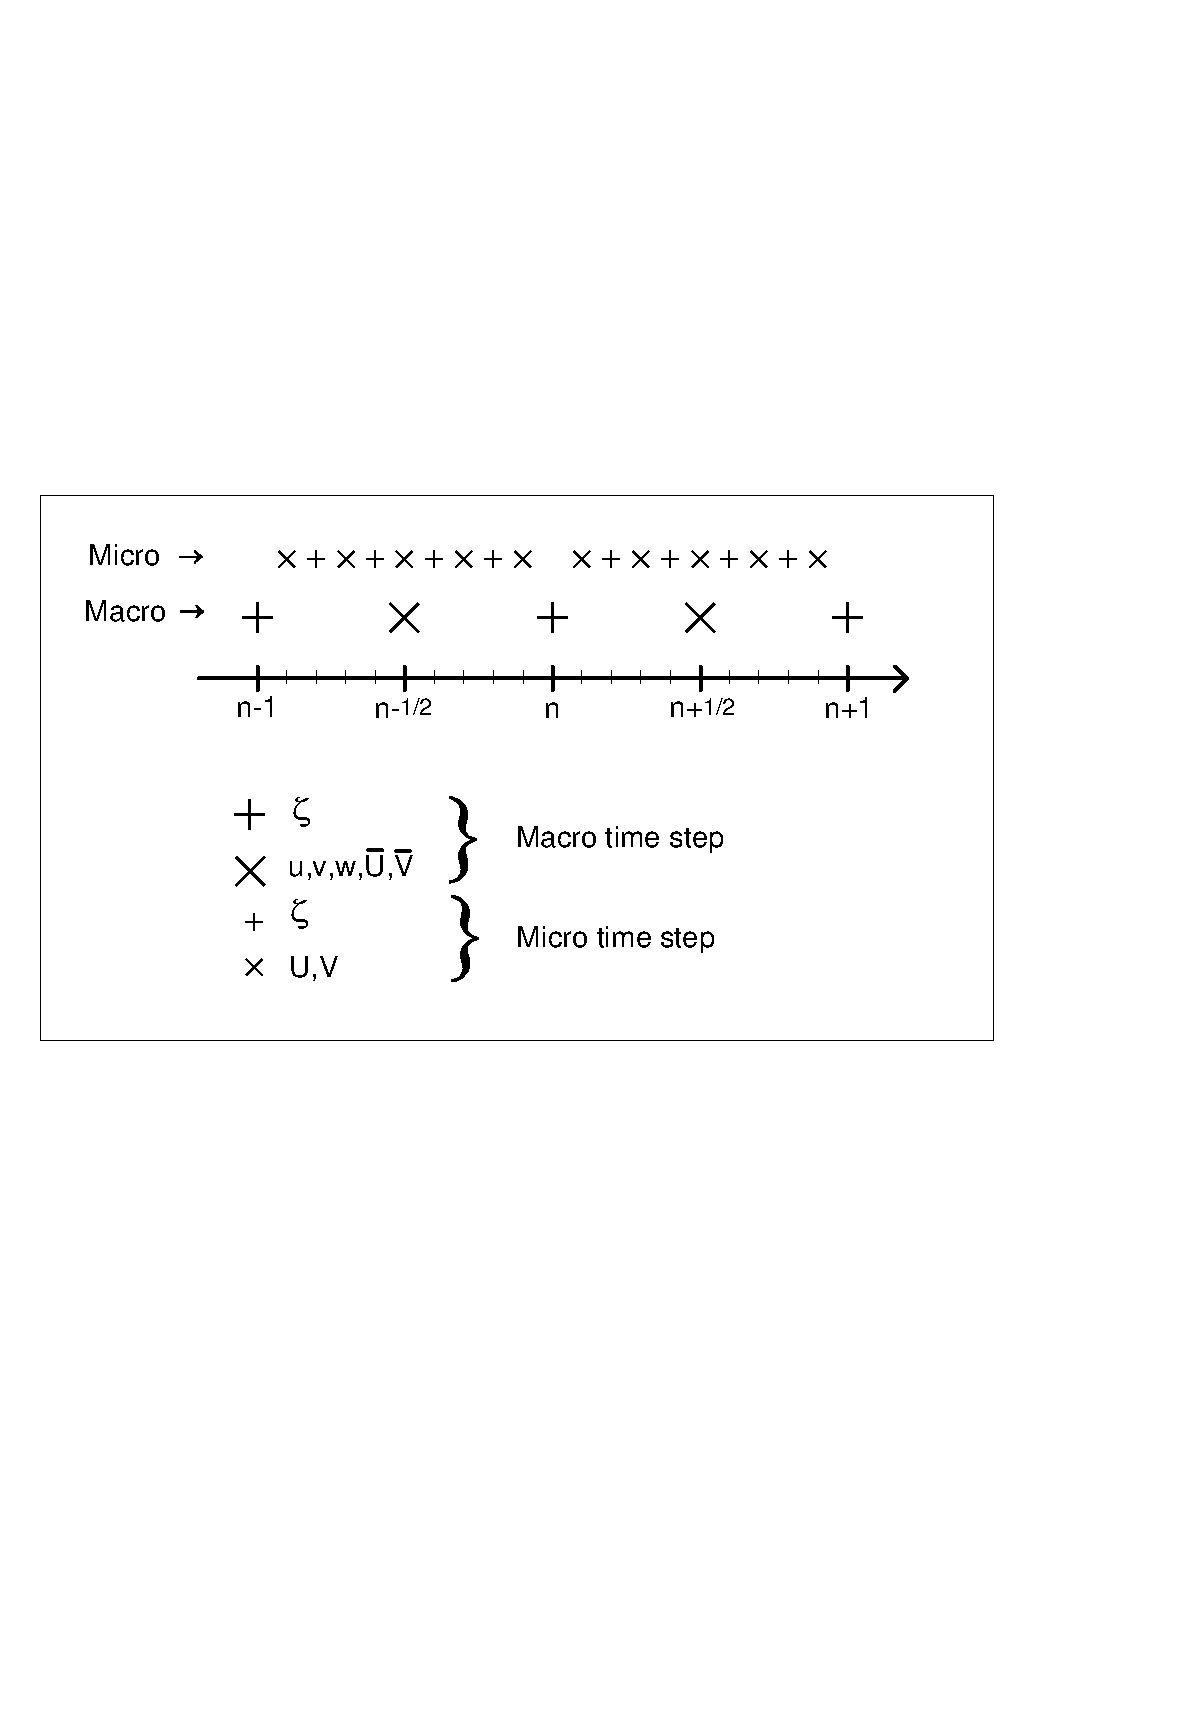
\includegraphics[width=12cm,bbllx=20,bblly=327,bburx=493,bbury=605]{./figures/gridtime.ps}
\caption{Sketch explaining the organisation of the time stepping.
}\label{figtimegrid}
\end{center}
\end{figure}


\subsection{Spatial discretisation}\label{Section_spatial_discretisation}


\begin{figure}
\begin{center}
\fbox{
\includegraphics[width=12cm,bbllx=126,bblly=462,bburx=513,bbury=714]{./figures/Picsh.ps}
}
\caption{Layout of the model horizontal model grid
in Cartesian coordinates. Shown are the
reference boxes for the T-points. The following symbols are used:
$+$: T-points; $\times$: U-points; $\star$: V-points; $\bullet$: X-points.
The inserted box denotes grid points with the same index $(i,j)$.}
\label{fighorgrid}
\end{center}
\end{figure}

For the spatial discretisation, a staggered C-grid is used, see 
\cite{ARAKAWAea77}.  
The grid consists of prism-shaped finite volumes with the
edges aligned with coordinates. The reference grid for the tracer
points (from now on denoted by T-points) is shown in figures 
\ref{fighorgrid} and \ref{figvertgrid}. The velocity points are located such
that the corresponding velocity components are centralised on the 
surfaces of the T-point reference box, the $u$-velocity points (from now on
U-points) at the western and eastern surfaces, the $v$-velocity
points (from now on V-points) at the southern and northern surfaces and the  
$w$-velocity
points (from now on W-points) at the lower and upper surfaces.
The indexing is carried out with $i$-indices\label{indexi} 
in eastern (${\cal X}$-) 
direction, 
with $j$-indices\label{indexj} 
in northern (${\cal Y}$-) direction and with $k$-indices
in upward ($z$-) direction, such that each grid point is identified
by a triple $(i,j,k)$. A T-point and the corresponding eastern U-point,
the northern V-point and the above W-point have always the same index,
see figures \ref{fighorgrid} and \ref{figvertgrid}.
The different grid points cover the following index ranges:

\begin{equation}\label{imaxjmax}
\begin{array}{llll}
\mbox{T-points:} & 1 \leq i \leq i_{\max}, & 
                   1 \leq j \leq j_{\max}, &
		   1 \leq k \leq k_{\max} \\
\mbox{U-points:} & 0 \leq i \leq i_{\max}, & 
                   1 \leq j \leq j_{\max}, &
		   1 \leq k \leq k_{\max} \\
\mbox{V-points:} & 1 \leq i \leq i_{\max}, & 
                   0 \leq j \leq j_{\max}, &
		   1 \leq k \leq k_{\max} \\
\mbox{W-points:} & 1 \leq i \leq i_{\max}, & 
                   1 \leq j \leq j_{\max}, &
		   0 \leq k \leq k_{\max} 
\end{array}
\end{equation}

On the T-points, all tracers such as\label{TSfirst} 
temperature $T$, salinity $S$,
the general tracers $c^i$ and the density are located. All turbulent
quantities such as eddy viscosity $\nu_t$ and eddy diffusivity $\nu_t'$
are located on the W-points.


\begin{figure}
\begin{center}
\psfrag{A}[lc][][1.4]{$(x_{i-1,j},y_{i-1,j})$}
\psfrag{B}[lc][][1.4]{$(x_{i,j},y_{i,j})$}
\psfrag{C}[lc][][1.4]{$(x_{i,j-1},y_{i,j-1})$}
\psfrag{D}[lc][][1.4]{$(x_{i-1,j-1},y_{i-1,j-1})$}
\includegraphics[width=8cm,bbllx=50,bblly=50,bburx=543,bbury=556]{./figures/CurviDXDY.ps}
\caption{Grid layout and indexing of corner points for
curvilinear grids. }
\label{fighorgridCurvi}
\end{center}
\end{figure}

For curvilinear grids, several arrays for spatial
increments $\Delta x$ and $\Delta y$  have to be defined:  

\begin{equation}\label{dxdycuv+}
\begin{array}{rcl}
\Delta x^c_{i,j}&=&\left|\left|
\frac12(X_{i,j-1}+X_{i,j}-X_{i-1,j-1}-X_{i-1,j}) 
\right|\right|\\ \\
\Delta x^u_{i,j}&=&\left|\left|
\frac14(X_{i+1,j-1}+X_{i+1,j}-X_{i-1,j-1}-X_{i-1,j})\right|\right| \\ \\
\Delta x^v_{i,j}&=& \left|\left|X_{i,j}-X_{i-1,j}\right|\right| \\ \\
\Delta x^+_{i,j}&=&\left|\left|
\frac12(X_{i+1,j}-X_{i-1,j})\right|\right| \\ \\
\Delta y^c_{i,j}&=&\left|\left|
\frac12(X_{i-1,j}+X_{i,j}-X_{i-1,j-1}-X_{i,j-1})\right|\right| \\ \\
\Delta y^u_{i,j}&=&\left|\left|X_{i,j}-X_{i,j-1}\right|\right|
 \\ \\
\Delta y^v_{i,j}&=&\left|\left|
\frac14(X_{i-1,j+1}+X_{i,j+1}-X_{i-1,j-1}-X_{i,j-1})\right|\right| \\ \\
\Delta y^+_{i,j}&=&\left|\left|
\frac12(X_{i,j+1}-X_{i,j-1})\right|\right| \\ \\
\end{array} 
\end{equation}

where $\left|\left|X_{i,j}-X_{i-1,j}\right|\right|
=\left((x_{i,j}-x_{i-1,j})^2+(y_{i,j}-y_{i-1,j})^2\right) ^{1/2}$.
The superscripts $c,u,v,+$ in (\ref{dxdycuv+}) indicate whether a $\Delta x$ or
$\Delta y$ is centrered at a T-, U-, V-, or X-point, respectively.  
For the locations of the corner points $X_{i,j}=(x_{i,j},y_{i,j})$, 
see figure \ref{fighorgridCurvi}. 


\subsection{Lateral boundary conditions}

Usually, a land mask is defined on the horizontal numerical grid.
This mask is denoted by $a^z$\label{az} for T-points, $a^u$\label{au} 
for U-points
and $a^v$\label{av} 
for V-points with $a^z$, $a^u$, and $a^v$ being integer fields. 
A T-point is either a land point ($a^z=0$) or a water point ($a^z>0$).
All U- and V-points surrounding a land point are defined as
closed boundary and masked out: $a^u=0$ and $a^v=0$.
The velocities on such closed boundaries are always set to 0.

Open boundaries are defined by $a^z>1$ for T-points.
Forced boundary points are marked by $a^z=2$ and passive
boundary points by $a^z=3$. 
All other T-points are characterised by $a^z=1$. 
For velocity points, three different types are defined at the
open boundaries. U-points are classified by $a^u=3$ if both 
the T-points east and west are open boundary points and by $a^u=2$
if one adjacent T-point is an open boundary point and the other 
an open water point with $a^z=1$. The same
is carried out for V-points: They are classified by $a^v=3$ if both
the T-points south and north are open boundary points and by $a^v=2$
if one adjacent T-point is an open boundary point
and the other an open water point with $a^z=1$.
U-points which are adjacent to T-points with $a^z=2$ and
which are not denoted by $a^u=2$ or $a^u=3$ are the external U-points
and are denoted by $a^u=4$. The same holds for V-points:
Those which are adjacent to T-points with $a^z=2$ and
which are not denoted by $a^v=2$ or $a^v=3$ are the external V-points
and are denoted by $a^v=4$.

\begin{figure}
\begin{center}
\fbox{
\includegraphics[width=12cm,bbllx=126,bblly=462,bburx=513,bbury=754]{./figures/Picsv.ps}
}
\caption{Layout of the model vertical model grid through the U-points. 
Shown are the
reference boxes for the T-points. The following symbols are used:
$+$: T-points; $\times$: U-points; $\triangle$: W-points; $\circ$: X$^u$-points.
The inserted box denotes grid points with the same index $(i,k)$.
The grid in the $(j,k)$-plane through the V-points is equivalent.}
\label{figvertgrid}
\end{center}
\end{figure}

For a simple example of grid point classification, see figure 
\ref{mask}.

\setlength{\unitlength}{1.5cm}
\begin{figure}
\begin{center}
\fbox{
\begin{picture}(6.0,6.0)(-0.5,-0.5)
\dottedline{0.1}(0,0)(0,5)
\dottedline{0.1}(1,0)(1,5)
\dottedline{0.1}(2,0)(2,5)
\dottedline{0.1}(3,0)(3,5)
\dottedline{0.1}(4,0)(4,5)
\dottedline{0.1}(5,0)(5,5)
\dottedline{0.1}(0,0)(5,0)
\dottedline{0.1}(0,1)(5,1)
\dottedline{0.1}(0,2)(5,2)
\dottedline{0.1}(0,3)(5,3)
\dottedline{0.1}(0,4)(5,4)
\dottedline{0.1}(0,5)(5,5)
\put(0.5,0.5){\makebox(0,0)[c]{\large\bf 2}}
\put(0.5,1.5){\makebox(0,0)[c]{\large\bf 2}}
\put(0.5,2.5){\makebox(0,0)[c]{\large\bf 2}}
\put(0.5,3.5){\makebox(0,0)[c]{\large\bf 2}}
\put(0.5,4.5){\makebox(0,0)[c]{\large\bf 0}}
\put(1.5,0.5){\makebox(0,0)[c]{\large\bf 2}}
\put(1.5,1.5){\makebox(0,0)[c]{\large\bf 1}}
\put(1.5,2.5){\makebox(0,0)[c]{\large\bf 1}}
\put(1.5,3.5){\makebox(0,0)[c]{\large\bf 1}}
\put(1.5,4.5){\makebox(0,0)[c]{\large\bf 0}}
\put(2.5,0.5){\makebox(0,0)[c]{\large\bf 2}}
\put(2.5,1.5){\makebox(0,0)[c]{\large\bf 1}}
\put(2.5,2.5){\makebox(0,0)[c]{\large\bf 1}}
\put(2.5,3.5){\makebox(0,0)[c]{\large\bf 1}}
\put(2.5,4.5){\makebox(0,0)[c]{\large\bf 0}}
\put(3.5,0.5){\makebox(0,0)[c]{\large\bf 2}}
\put(3.5,1.5){\makebox(0,0)[c]{\large\bf 1}}
\put(3.5,2.5){\makebox(0,0)[c]{\large\bf 1}}
\put(3.5,3.5){\makebox(0,0)[c]{\large\bf 1}}
\put(3.5,4.5){\makebox(0,0)[c]{\large\bf 0}}
\put(4.5,0.5){\makebox(0,0)[c]{\large\bf 0}}
\put(4.5,1.5){\makebox(0,0)[c]{\large\bf 0}}
\put(4.5,2.5){\makebox(0,0)[c]{\large\bf 0}}
\put(4.5,3.5){\makebox(0,0)[c]{\large\bf 0}}
\put(4.5,4.5){\makebox(0,0)[c]{\large\bf 0}}
\put(0,0.5){\makebox(0,0)[c]{\large\bf 4}}
\put(0,1.5){\makebox(0,0)[c]{\large\bf 4}}
\put(0,2.5){\makebox(0,0)[c]{\large\bf 4}}
\put(0,3.5){\makebox(0,0)[c]{\large\bf 4}}
\put(0,4.5){\makebox(0,0)[c]{\large\bf 0}}
\put(1,0.5){\makebox(0,0)[c]{\large\bf 3}}
\put(1,1.5){\makebox(0,0)[c]{\large\bf 2}}
\put(1,2.5){\makebox(0,0)[c]{\large\bf 2}}
\put(1,3.5){\makebox(0,0)[c]{\large\bf 2}}
\put(1,4.5){\makebox(0,0)[c]{\large\bf 0}}
\put(2,0.5){\makebox(0,0)[c]{\large\bf 3}}
\put(2,1.5){\makebox(0,0)[c]{\large\bf 1}}
\put(2,2.5){\makebox(0,0)[c]{\large\bf 1}}
\put(2,3.5){\makebox(0,0)[c]{\large\bf 1}}
\put(2,4.5){\makebox(0,0)[c]{\large\bf 0}}
\put(3,0.5){\makebox(0,0)[c]{\large\bf 3}}
\put(3,1.5){\makebox(0,0)[c]{\large\bf 1}}
\put(3,2.5){\makebox(0,0)[c]{\large\bf 1}}
\put(3,3.5){\makebox(0,0)[c]{\large\bf 1}}
\put(3,4.5){\makebox(0,0)[c]{\large\bf 0}}
\put(4,0.5){\makebox(0,0)[c]{\large\bf 0}}
\put(4,1.5){\makebox(0,0)[c]{\large\bf 0}}
\put(4,2.5){\makebox(0,0)[c]{\large\bf 0}}
\put(4,3.5){\makebox(0,0)[c]{\large\bf 0}}
\put(4,4.5){\makebox(0,0)[c]{\large\bf 0}}
\put(5,0.5){\makebox(0,0)[c]{\large\bf 0}}
\put(5,1.5){\makebox(0,0)[c]{\large\bf 0}}
\put(5,2.5){\makebox(0,0)[c]{\large\bf 0}}
\put(5,3.5){\makebox(0,0)[c]{\large\bf 0}}
\put(5,4.5){\makebox(0,0)[c]{\large\bf 0}}
\put(0.5,0){\makebox(0,0)[c]{\large\bf 4}}
\put(0.5,1){\makebox(0,0)[c]{\large\bf 3}}
\put(0.5,2){\makebox(0,0)[c]{\large\bf 3}}
\put(0.5,3){\makebox(0,0)[c]{\large\bf 3}}
\put(0.5,4){\makebox(0,0)[c]{\large\bf 0}}
\put(0.5,5){\makebox(0,0)[c]{\large\bf 0}}
\put(1.5,0){\makebox(0,0)[c]{\large\bf 4}}
\put(1.5,1){\makebox(0,0)[c]{\large\bf 2}}
\put(1.5,2){\makebox(0,0)[c]{\large\bf 1}}
\put(1.5,3){\makebox(0,0)[c]{\large\bf 1}}
\put(1.5,4){\makebox(0,0)[c]{\large\bf 0}}
\put(1.5,5){\makebox(0,0)[c]{\large\bf 0}}
\put(2.5,5){\makebox(0,0)[c]{\large\bf 0}}
\put(2.5,0){\makebox(0,0)[c]{\large\bf 4}}
\put(2.5,1){\makebox(0,0)[c]{\large\bf 2}}
\put(2.5,2){\makebox(0,0)[c]{\large\bf 1}}
\put(2.5,3){\makebox(0,0)[c]{\large\bf 1}}
\put(2.5,4){\makebox(0,0)[c]{\large\bf 0}}
\put(2.5,5){\makebox(0,0)[c]{\large\bf 0}}
\put(3.5,0){\makebox(0,0)[c]{\large\bf 4}}
\put(3.5,1){\makebox(0,0)[c]{\large\bf 2}}
\put(3.5,2){\makebox(0,0)[c]{\large\bf 1}}
\put(3.5,3){\makebox(0,0)[c]{\large\bf 1}}
\put(3.5,4){\makebox(0,0)[c]{\large\bf 0}}
\put(3.5,5){\makebox(0,0)[c]{\large\bf 0}}
\put(4.5,0){\makebox(0,0)[c]{\large\bf 0}}
\put(4.5,1){\makebox(0,0)[c]{\large\bf 0}}
\put(4.5,2){\makebox(0,0)[c]{\large\bf 0}}
\put(4.5,3){\makebox(0,0)[c]{\large\bf 0}}
\put(4.5,4){\makebox(0,0)[c]{\large\bf 0}}
\put(4.5,5){\makebox(0,0)[c]{\large\bf 0}}
\end{picture}
}
\caption{Classification of grid points for a simple $5 \times 5$ 
configuration ($i_{\max}=j_{\max}=5$). 
On the locations for T-, U- and V-points, the values
of $a^z$, $a^u$, and $a^v$, respectively, are written.
The northern and eastern boundaries are closed and the western and southern
boundaries are open and forced. }
\label{mask}
\end{center}
\end{figure}


When the barotropic boundary forcing is carried out by means of 
prescribed surface elevations only, then the surface elevation $\zeta$
is prescribed in all T-points with $a^z=2$. 
For passive boundary conditions ($a^z=3$), where the curvature of the 
surface elevation is zero normal to the boundary, the surface 
slope is simply extrapolated to the boundary points. For a boundary point
$(i,j)$ at the western boundary this results e.g.\ in the
following calculation for the boundary point:

\begin{equation}
\zeta_{i,j}=\zeta_{i+1,j}+(\zeta_{i+1,j}-\zeta_{i+2,j})=
2\zeta_{i+1,j}-\zeta_{i+2,j}. 
\end{equation}


\subsection{Bed friction}\label{SectionBedFric}
 
As already mentioned earlier in section \ref{SectionDynBounds},
caution is needed when discretising the
bottom boundary conditions for momentum, (\ref{DynBoundbx}).
They are an example
for a physical condition which has to be modified for the numerical
discretisation, since the discrete velocity point nearest to the bottom
is half a grid box away from the point where the
\index{boundary conditions}boundary condition
is defined. Furthermore, due to the logarithmic \index{law of the wall}
law, high velocity
gradients are typical near the bed. Simply setting the discrete bottom
velocity to zero, would therefore lead to large discretisation errors.
Instead, a flux condition using bottom stresses is derived from the 
law of the wall.

For the determination of the normalised bottom stresses

\begin{equation}\label{tauxb}
\frac{\tau^x_b}{\rho_0}=u_*^{bx}u_*^b,
\end{equation}
\begin{equation}\label{tauyb}
\frac{\tau^y_b}{\rho_0}=u_*^{by}u_*^b
\end{equation}

with the friction velocities
$u_*^b=\sqrt{\tau_b/\rho_0}$\label{pagetaub} with
$\tau_b=\sqrt{(\tau^x_{b})^2+(\tau^y_{b})^2}$,
assumptions about the structure of
velocity inside the discrete bottom layer have to be made.
We use here the logarithmic profile 

\begin{equation}\label{log_prof}
\frac{u(z')}{u_*}
=\frac{1}{\kappa}\mbox{ln}\left(\frac{z'+z_0^b}{z_0^b}\right),
\end{equation}

with the bottom roughness length $z_0^b$, the von K\'arm\'an constant $\kappa=0.4$
and the distance from the bed, $z'$. 
Therefore, estimates for the velocities in the centre of the bottom
layer can be achieved by:

\begin{equation}\label{ulogdis}
u_b = \frac{u_*^{bx}}{\kappa}\mbox{ln} \left(\frac{0.5h_1+z_0^b}{z_0^b}\right),
\end{equation}

\begin{equation}\label{vlogdis}
v_b = \frac{u_*^{by}}{\kappa}\mbox{ln} \left(\frac{0.5h_1+z_0^b}{z_0^b}\right).
\end{equation}

For $h_1\rightarrow 0$, the original \index{boundary conditions!Dirichlet-type}
Dirichlet-type
no-slip boundary conditions (\ref{DynBoundbx}) are retained.
Another possibility would be to specify the bottom velocities $u_b$ and $v_b$
such that they are equal to the layer-averaged \index{law of the wall}
log-law velocities
(see \cite{BAUMERTea92}).
The calculation of this is however slightly more time consuming
and does not lead to a higher accuracy.



\subsection{Drying and flooding}\label{Section_dry}

The main requirement for drying and flooding is that the
vertically integrated fluxes $U$ and $V$ are controlled such
that at no point a negative water depth occurs.
It is clear that parts of the physics which
play an important role in very shallow water of a
few centimetres depth
like non-hydrostatic effects
are not included in the equations.
However, the model is designed in a way that the control of $U$ and $V$
in very shallow water is mainly motivated by the physics
included in the equations
rather than by defining complex drying and flooding algorithms.
It is assumed that the major process in this
situation is a balance between pressure gradient and bottom friction.
Therefore, in the case of very shallow water, all other terms are multiplied
with the non-dimensional factor $\alpha$ which approaches zero
when a minimum water depth is reached.

By using formulation (\ref{bottom_vert})
for calculating the bottom drag coefficient $R$,
it is guaranteed that $R$ is exponentially growing if the water depth
approaches very small values.
This slows the flow down when the water depth in a
velocity point is sinking and also allows for flooding without
further manipulation.

\setlength{\unitlength}{0.5cm}
\begin{figure}
\begin{center}
\fbox{
\begin{picture}(23.0,21.0)(-2.5,-0.5)
\thinlines
\drawline[0](4,8)(4,18)
\drawline[0](10,8)(10,18)
\drawline[0](16,8)(16,18)
\thicklines
\drawline[0](4,15)(10,15)(10,8)(16,8)
\drawline[0](4,15.05)(10.05,15.05)(10.05,8.05)(16,8.05)
\drawline[0](4,14.95)(9.95,14.95)(9.95,7.95)(16,7.95)
\thinlines
\drawline[0](4,16.3)(10,16.3)
\drawline[0](10,11)(16,11)
\dashline[+50]{0.2}(4,16.6)(16,16.6)
\dashline[+50]{0.2}(3,6)(7,6)
\drawline[0](3,4.5)(7,4.5)
\thicklines
\drawline[0](3,3)(7,3)
\drawline[0](3,2.95)(7,2.95)
\drawline[0](3,3.05)(7,3.05)
\put(8,6){\makebox(0,0)[l]{Virtual sea surface elevation}}
\put(8,4.5){\makebox(0,0)[l]{Actual sea surface elevation}}
\put(8,3){\makebox(0,0)[l]{Bathymetry approximation}}
\thinlines
\drawline[10](4,15)(3,14)
\put(2.8,14){\makebox(0,0)[r]{$-H_{i,j}$}}
\drawline[10](4,16.3)(3,16.3)
\put(2.8,16.3){\makebox(0,0)[r]{$\zeta_{i,j}$}}
\drawline[10](4,16.6)(3,17.6)
\put(2.8,17.6){\makebox(0,0)[r]{$-H_{i,j}+H_{\min}$}}
\drawline[10](16,16.6)(17,16.6)
\put(17.2,16.6){\makebox(0,0)[l]{$\tilde \zeta_{i+1,j}$}}
\drawline[10](16,11)(17,11)
\put(17.2,11){\makebox(0,0)[l]{$\zeta_{i+1,j}$}}
\drawline[10](16,8)(17,8)
\put(17.2,8){\makebox(0,0)[l]{$-H_{i+1,j}$}}
\end{picture}
}
\caption{
Sketch explaining the principle of pressure gradient
minimisation during drying and flooding over sloping bathymetry.
}
\label{figpressgrad}
\end{center}
\end{figure}

In this context, one important question is how to calculated the depth 
in the velocity points, $H^u$ and $H^v$, since this determines how shallow the
water in the velocity points may become on sloping beaches. 
In ocean models, usually, the depth in the velocity points is calculated as
the mean of depths in adjacent elevation points (T-points):

\begin{equation}\label{Hmean}
H^u_{i,j}=\frac12\left(H_{i,j}+H_{i+1,j}\right),
\qquad
H^v_{i,j}=\frac12\left(H_{i,j}+H_{i,j+1}\right).
\end{equation}

Other models which deal with drying and flooding such as the models of
\cite{DUWE88} and \cite{CASULLIea94} use the minimum of the adjacent depths in
the T-points:

\begin{equation}\label{Hmin}
H^u_{i,j}= \min\{H_{i,j},H_{i+1,j}\},
\qquad
H^v_{i,j}= \min\{H_{i,j},H_{i,j+1}\}.
\end{equation}

This guarantees that all depths in the velocity points around a T-point are not
deeper than the depth in the T-point. 
Thus, when the T-point depth is approaching
the minimum depth, then all depths in the velocity 
points are also small and the
friction coefficient correspondingly large. 

Each of the methods has however drawbacks: When the mean is taken as in
(\ref{Hmean}), the risk of negative water depths is relatively big, and thus
higher values of $D_{\min}$ have to be chosen. When the minimum is taken, 
large mud-flats might need unrealistically long times for drying since all
the water volume has to flow through relatively shallow velocity boxes.
Also, velocities in these shallow boxes tend to be relatively high in order to
provide sufficient transports. This might lead to numerical instabilities. 

Therefore, GETM has both options, (\ref{Hmean}) and (\ref{Hmin}) 
and the addition of various other options such
as depth depending weighting of the averaging can easily be added.  
These options are controlled by the GETM variable {\tt vel\_depth\_method},
see section \ref{sec-uv-depth} (subroutine {\tt uv\_depths}) documented
on page \pageref{sec-uv-depth}.

If a pressure point is dry (i.e.\ its bathymetry value is higher than
a neighbouring sea surface elevation),
the pressure gradient would be unnaturally high with the consequence
of unwanted flow acceleration. Therefore this pressure gradient will
be manipulated such that (only for the pressure gradient calculation)
a virtual sea surface elevation $\tilde \zeta$ is assumed
(see figure \ref{figpressgrad}). In the situation shown in figure
\ref{figpressgrad}, the left pressure point is dry, and the sea surface
elevation
there is for numerical reasons even slightly below the critical value
$-H_{i,j}+H_{\min}$. In order not to let more water flow out of the left cell,
the pressure gradient between the two boxes shown is calculated with a
manipulated sea surface elevation on the right, $\tilde \zeta_{i+1,j}$.

See also \cite{BURCHARDea03a} for a description of drying and flooding 
numerics in GETM.

